\section{Supplement: the final windows of the first version}
\label{sec:supplementfinal}

The first version of this paper scored each data set once, on its final window,
with three seeds per trained model. These results come before the rolling
windows of the main text and are kept here for the record.


\input{generated/tab_m5}
\input{generated/tab_finals}
\input{generated/rev_tab_finalsnew}

The first version scored each data set once, on its final window, and its
findings stand: on M5 the most accurate model depended on the level and the
month (Table~\ref{tab:m5}), and on Dominick's and Frat on the category
(Table~\ref{tab:finals}). On M5, TimesFM given only history was the most
accurate single model item by store in all four months (\mTfmTestIxs{} on the
test month, against \mWorldTestIxs{} for the world model and \mLgbTestIxs{} for
LightGBM), while the plan-aware models were far more accurate at the totals. The
official test month was the only one of four in which LightGBM was the most
accurate over all levels (\mLgbTestOverall{} against \mWorldTestOverall), so a
comparison on that month alone would have ranked it first. Run on the final
windows (Table~\ref{tab:finalsnew}), the ensemble is lowest or within
\rcount{finalsgap} of the lowest item by store on every data set, which agrees
with the rolling windows.
One final run did not finish as first started: the frozen-entrees world model,
seed 3, stopped when the runtime dropped, could not be resumed because of a
fault in restoring its random state (since fixed), and was run again from the
start with the same settings (0.476 overall).

\begin{figure*}[t]
\centering
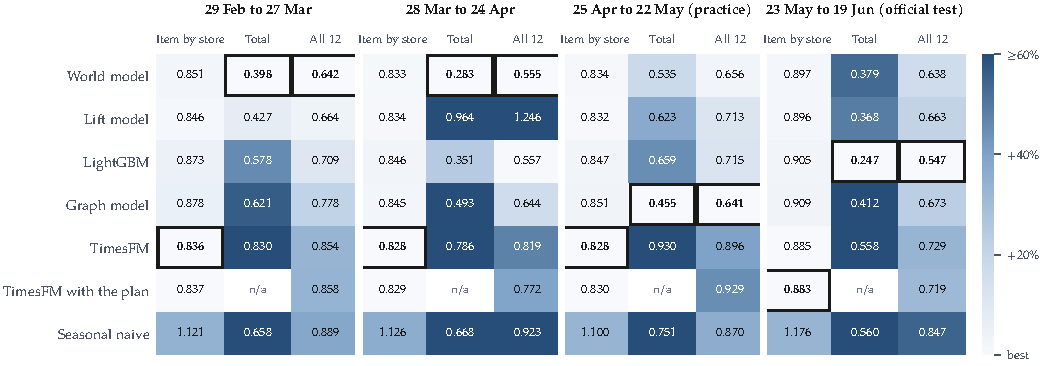
\includegraphics[width=\textwidth]{figs/fig_m5_heat.pdf}
\caption{\textbf{On the M5 final windows, TimesFM from history alone had the
lowest item-by-store error of the single models in every month; at the total and
over all levels the plan-aware models did, and which one changed by month.}
WRMSSE of every single model, four windows, three levels; cell shade: how far
above the lowest value in its column (white: the lowest, outlined). Trained
models: mean of three seeds. The lift model's April mean includes one failed
seed (\S\ref{sec:dropped-first}).}
\label{fig:m5heat}
\end{figure*}

\paragraph{How much the plan matters}
On M5, where prices rarely change, giving TimesFM the plan changed its
item-by-store error by at most 0.002 in any month. On Dominick's, where promoted
weeks carry \promoShareLo\% to \promoShareHi\% of a category's units, TimesFM
without the plan forecast \promoTfmLo\% to \promoTfmHi\% of promoted-week sales
and with it \promoTfmPlanLo\% to \promoTfmPlanHi\%
(Figure~\ref{fig:planarrows}a). The trained plan-aware models also fell short in
promoted weeks: the world model forecast \promoWorldLo\% to \promoWorldHi\% of
promoted-week sales and LightGBM \promoLgbLo\% to \promoLgbHi\%.

\begin{figure*}[t]
\centering
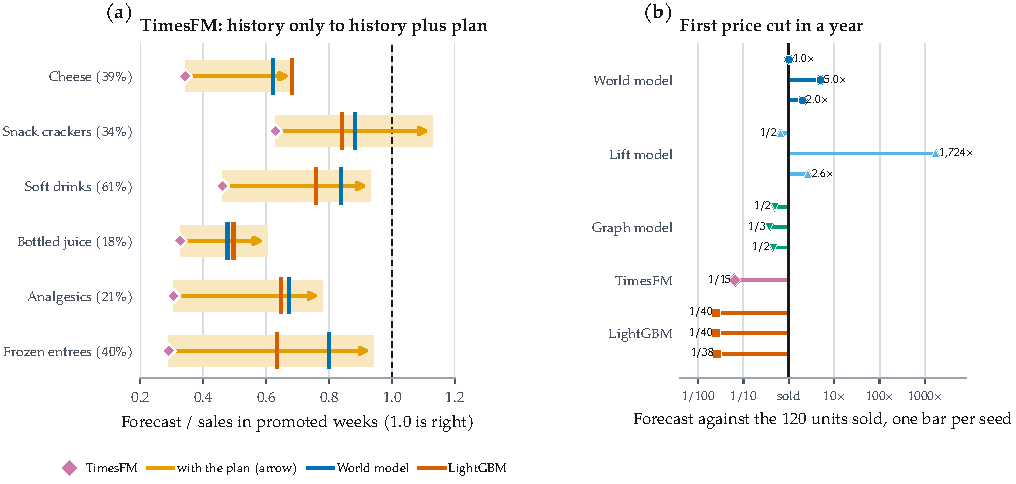
\includegraphics[width=\textwidth]{figs/fig_plan_arrows.pdf}
\caption{\textbf{Given the plan, TimesFM closes most of its promoted-week
shortfall; for a price cut history has not shown, plan-aware models respond and
history-only models do not.} \textbf{(a)} Forecast against sales in the promoted
weeks of the final 8 weeks, by Dominick's category (promoted weeks' share of the
category's units in brackets): TimesFM from history alone (diamond) to TimesFM
with the plan (arrow head), with the world model and LightGBM (ticks). \textbf{(b)}
HOUSEHOLD\_1\_146 in the four M5 stores where it had its first price cut in a year
(5.98 to 4.50 for one week) inside the April window: each seed's forecast over
the 28 days against the \cutSold{} units sold, log scale.}
\label{fig:planarrows}
\end{figure*}

\paragraph{First-time price cuts}
In the April M5 window, HOUSEHOLD\_1\_146 had sold almost nothing for a year at
5.98, then sold \cutSold{} units in four stores over a window that held a
one-week cut to 4.50 (Figure~\ref{fig:planarrows}b). Models working from history
forecast almost nothing: LightGBM \cutLgb{} units across seeds, TimesFM
\cutTfm. The world model, which reads the cut through its plan, forecast
\cutWorld; the graph model \cutGraph; the lift model \cutLift. How large the
response should be is not fixed by the data: the world-model seeds differ by a
factor of five, and one lift-model seed forecast over 200,000 units.

\paragraph{Items with no recent sales}
On M5 the error at the chain total followed the error in the overall level
(correlation \biasErrCorr{} over \biasErrN{} runs of every model on the four windows,
Figure~\ref{fig:levelscatter}a). Grouping April's item-stores by their sales in
March (Figure~\ref{fig:levelscatter}b), both models were within 6\% of sales in
every group that sold in March, and the world model was closer on 50.6\% to
54.2\% of item-stores in each. On item-stores that sold nothing in March, which
sold 14,102 units in April, the world model forecast 62\% too much and LightGBM
5\% too little: the world model's weakest group. A first grouping by sales in the
scored window itself had shown LightGBM's under-forecast growing with the sales
rate, to 18\% on the fastest items; that pattern came from grouping by the
outcome being scored and is not reported as a finding.

\begin{figure*}[t]
\centering
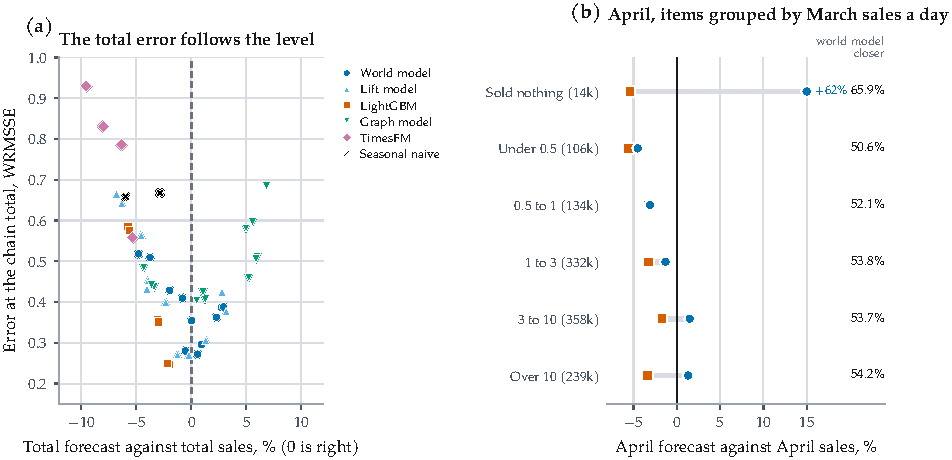
\includegraphics[width=\textwidth]{figs/fig_level_scatter.pdf}
\caption{\textbf{On M5 the error at the total followed the error in the level,
and the world model over-forecast item-stores that sold nothing the month
before.} \textbf{(a)} Total forecast against total sales and WRMSSE at the chain
total, every model and seed on the four M5 windows (the failed April lift seed
left out). \textbf{(b)} April forecast against April sales by the item-store's
sales a day in March (April units in brackets), world model and LightGBM, three
seeds averaged; right: the share of item-stores where the world model was
closer.}
\label{fig:levelscatter}
\end{figure*}


\subsection{What the first version tried and dropped}
\label{sec:dropped-first}

\input{generated/tab_ledger}

\paragraph{A lift-model seed that broke on five series}
In the April M5 final window, lift-model seed 2 scored \mLiftAprSeedBOverall{}
over all levels against \mLiftAprSeedAOverall{} and \mLiftAprSeedCOverall{} for
seeds 1 and 3, and forecast \liftSeedTwoForecast{} units against
\liftSeedTwoSold{} sold. Five item-store series hold all of the excess, each with
its first price cut in a year inside the window; the seed read the cuts as lifts
up to the model's bound. Item by store, weighted by dollar sales, the failure is
invisible (\mLiftAprIxs); at the totals it dominates. The world model did not
fail on these series in any seed.

\begin{figure*}[t]
\centering
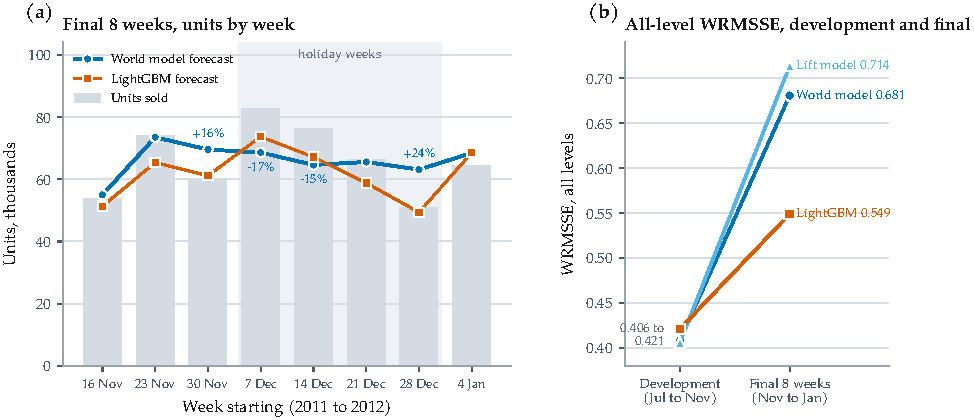
\includegraphics[width=\textwidth]{figs/fig_frat_story.pdf}
\caption{\textbf{On the Frat final window the world model got the 8-week total
right and missed the holiday shape, which the development windows did not
contain.} \textbf{(a)} Units sold each week of the final window over all
item-stores (bars), and the weekly forecasts of the world model and LightGBM,
three seeds averaged; labels: the world model's largest weekly misses.
\textbf{(b)} All-level WRMSSE on the development windows and on the final 8 weeks.}
\label{fig:fratstory}
\end{figure*}

\paragraph{Frat holiday weeks}
On the Frat development windows the world model, lift model and LightGBM were
level (0.406 to 0.421). On the final 8 weeks the world model fell to
\fWorldFratOverall{} against \fLgbFratOverall{} for LightGBM. The final weeks
are the holiday period, which the development windows did not contain
(Figure~\ref{fig:fratstory}); the world model's 8-week total is right (forecast
against sales \fWorldFratFa) but it is 15\% to 17\% under in the two December
peak weeks. LightGBM, with week-of-year and month inputs and the previous
holiday season in its training data, follows that shape more closely.

\paragraph{TimesFM's default output}
TimesFM's default point forecast is the median. For an item that sells nothing
on most days the median is near zero while the mean is not, so the median
forecast is 27\% to 31\% below M5 totals in every month. The mean output, used
throughout, does not have the problem.

